\documentclass[9pt,xcolor={dvipsnames}]{beamer}
\usepackage{algorithm}
\usepackage{algorithmic}
\usepackage{natbib}
\usepackage{tikz}
\usepackage[overload]{empheq}
\usepackage{empheq}
\usepackage{array, makecell}
\usepackage{tabularx}
\usepackage{caption}
\usepackage{rotating}
\usepackage{natbib}
\mode<presentation>{
	\usetheme{Warsaw}			%  http://www.hartwork.org/beamer-theme-matrix/
	\usecolortheme[named=Blue]{structure}
	\useoutertheme{shadow}
	\usefonttheme{professionalfonts} 	
	
	%\useoutertheme{sidebar}
	%\setbeamercolor*{sidebar}{fg=RoyalBlue,bg=!75!white}
	\setbeamercovered{transparent}
	\setbeamercolor{block title example}{fg=white,bg=Blue}
	\setbeamercolor{block body example}{fg=gray,bg=Blue!10}
	\setbeamercolor{postit1}{fg=white,bg=Blue}
	\setbeamercolor{postit2}{fg=gray,bg=Blue}
	\setbeamertemplate{itemize items}[default]
	\setbeamertemplate{enumerate items}[default]
	\setbeamertemplate{sections/subsections in toc}[sections numbered]
}

\makeatletter
\long\def\beamer@@ssection*#1{\beamer@section[]{}}
\makeatother
\newcommand{\RN}[1]{%
	\textup{\uppercase\expandafter{\romannumeral#1}}%
}
\usepackage{pgfpages}		% http://mathoverflow.net/questions/5893/beamer-printout
\mode<handout>{
	\usetheme{default}
	\setbeamercolor{background canvas}{bg=Gray!5}
	\pgfpagesuselayout{4 on 1}[a4paper,portrait,border shrink=2.5mm]		% 4 slide per pagina
}

%\usetheme{Boadila}
\usetheme{Warsaw}			%  http://www.hartwork.org/beamer-theme-matrix/
%\usecolortheme[named=RoyalBlue]{structure}
%\useoutertheme{shadow}
%\usefonttheme{professionalfonts} 			
%
%\usepackage{pgfpages}		% http://mathoverflow.net/questions/5893/beamer-printout
%\mode<handout>{
%  \usetheme{default}
%  \setbeamercolor{background canvas}{bg=Black!5}
%  \pgfpagesuselayout{4 on 1}[a4paper,portrait,border shrink=2.5mm]		% 4 slide per pagina
%}

\usepackage[english]{babel}
\usepackage[utf8x]{inputenc}
\usepackage{lmodern} 
\usepackage{times}
\usepackage[T1]{fontenc}
\usepackage{graphicx}
\usepackage{epstopdf}					   % immagini formato .eps
\graphicspath{{images/}}
\usepackage[export]{adjustbox}
\usepackage{adjustbox}
\usepackage{colortbl}
\usepackage{booktabs}                      % tabelle
\usepackage{tabularx}
\usepackage{etoolbox}
\usepackage[autostyle]{csquotes}		   % per le citazioni
\usepackage{eqnarray,amsmath,amssymb,amsthm}
\usepackage{xcolor}
\usepackage{multirow}
\usepackage[export]{adjustbox}
\usepackage{amsmath}
\usepackage{tikz}
\usetikzlibrary{shapes,arrows}
\tikzstyle{square}=[draw]
\usepackage{pgfplots}
\pgfplotsset{compat = newest}
\newcolumntype{P}[1]{>{\centering\arraybackslash}p{#1}}
\newcolumntype{M}[1]{>{\centering\arraybackslash}m{#1}}
\newcolumntype{C}[1]{>{\centering\arraybackslash}c{#1}}
\setbeamercovered{dynamic}

\hypersetup{
			pdftitle={Real-time optimization},
			%pdfsubject={},
			%pdfauthor={Ousmane Ali},
			pdfpagemode=FullScreen, % full screen
}

\usepackage[absolute,overlay]{textpos}
\setlength{\TPHorizModule}{1mm}
\setlength{\TPVertModule}{1mm}

%\begin{left}
  %\includegraphics[scale=0.1]{image/LavalLogo.jpg}\\[\bigskipamount]
%\end{left}
\begin{document}

\begin{center}
\vspace*{0.1cm}
 
\includegraphics[scale=0.15]{cirrelt.png}\\[\bigskipamount]
\end{center}

%\vspace{-1.2pt}
\vspace*{-2.2cm}
\title[Concrete transport optimization]{Real-time vehicle scheduling of a FTL transportation system}
\author[Ousmane Ali]{\textbf{Ousmane Ali\\ Jean-Fran\c{c}ois C\^ot{\'e} \\ Leandro C. Coelho}}

\date{}

\vspace{-0.5cm}
%\logo{\vspace{0.85cm}\includegraphics[height=0.8cm]{images/logo-universite-laval}} % logo in ogni pagina
%\titlegraphic{\vspace{0.85cm}
\includegraphics[height=0.8cm, angle=0, right]{images/cirrelt}} % immagine nella title page



\begin{frame}[noframenumbering]{}

\begin{center}
\vspace{-0.43651pt}
%\includegraphics[height=1.4cm, angle=0]{images/logo-polimi}
\titlepage

{\vspace*{-3cm}
	\texorpdfstring{
		\vspace{0.5cm}
		Université Laval \\
		\vspace{0.2cm}
		Département d'Opérations et Systèmes de Décision \\
		\centering
		\vspace*{0.3cm}
		December 7th, 2020
		\vspace*{1.5cm}
	}
	{}
}
\vspace{-3cm}
\end{center}

\end{frame}
\logo{}


\setbeamertemplate{footline}{%		% numerazione pagine
\vskip-4pt%
  \leavevmode%
  \hbox{\begin{beamercolorbox}[wd=.5\paperwidth,ht=2.5ex,dp=1.125ex,leftskip=.2cm plus1fill,rightskip=.2cm]{author in head/foot}%
    \usebeamerfont{author in head/foot}\insertshortauthor
  \end{beamercolorbox}%
  \begin{beamercolorbox}[wd=.5\paperwidth,ht=2.5ex,dp=1.125ex,leftskip=.3cm,rightskip=.3cm plus1fil]{title in head/foot}%
    \usebeamerfont{title in head/foot}\insertshorttitle
    ~~~\raggedleft\insertframenumber/\inserttotalframenumber
  \end{beamercolorbox}}%
  \vskip0pt%
}

\begin{frame}{Outline}
	\tableofcontents[hidesubsections]
\end{frame}

\section{Introduction}


\subsection{Context of the problem}
\begin{frame}{Cement  industry in Canada}
\setbeamercolor{block title}{use=structure,fg=white,bg=red!75!black}
\begin{block}{ }
\begin{itemize}
% \item 14 factories.
\item 13 million of tonnes of cement. 
\item 1.6 billion \$ of production. \footnote{\label{1} 2014}
\item Wide variety of products:   cement, concrete (UNISOLANT, UNIGEL, UNIPLAN, AGRIMIX, UNIFLOW)


\end{itemize}
\vspace{0.1cm}
\begin{center}
	
\includegraphics[scale=0.2]{ciment_quebec.jpg}
	
\includegraphics[scale=0.2]{Lafarge-logo.jpg}
	
\includegraphics[scale=0.2]{st-marys.jpg}
	
\includegraphics[scale=0.2]{mc-innis.png}
\end{center}
\end{block}

\end{frame}


\begin{frame}{Issues for concrete deliveries}
\setbeamercolor{block title}{use=structure,fg=white,bg=red!75!black}
\begin{block}{ }

\includegraphics[scale=0.5]{Unibeton.jpg}
\begin{itemize}
\item Hundred thousands deliveries per year.
\item Specialized workforce to drive the concrete-mixer.
	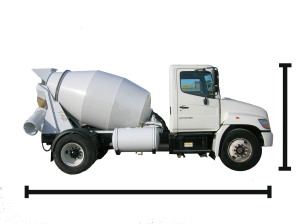
\includegraphics[scale=0.5]{betonniere.jpg}
\vspace{0.1cm}
\item Highly dynamic, perishable and seasonal demand.
\item Restrictions on deliverymen weekly work time.
\item High operating costs.
\item Weather dependent activities.
\end{itemize}
\end{block}
\end{frame}


\section{Problem description}

\begin{frame}{Flowchart}

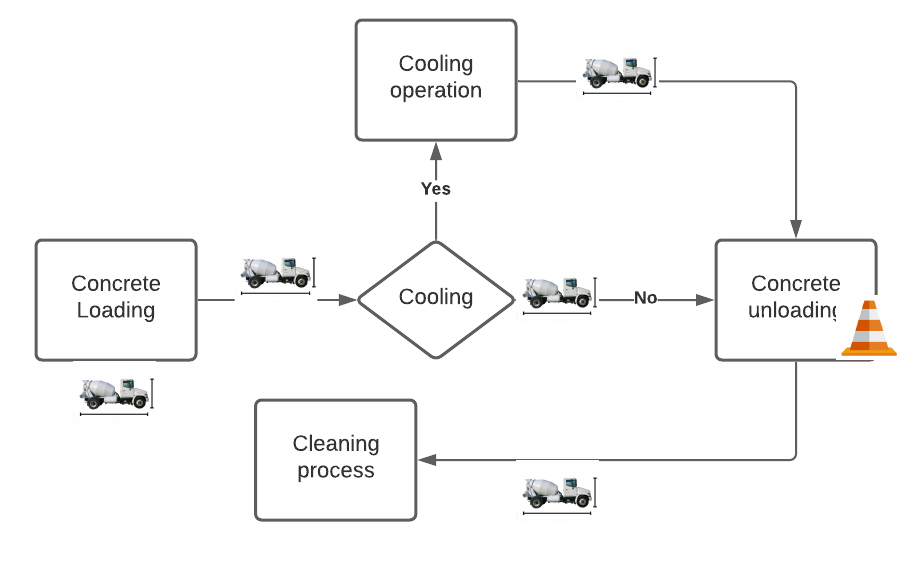
\includegraphics[scale=0.7]{flowchart.png}

\end{frame}

\begin{frame}{Problem description}

\begin{block}{Constraints (1)}
\begin{itemize}
\item Loading operation
	\begin{itemize}
		\item One vehicle at a time
		\item Loading time dependent of the type of concrete
		\item Additional cooling operation for some product.
	\end{itemize}
\item Transit time dependent of the road traffic.

\item Delivery at due time (synchronization with other services at the customer location).

\item Demand of a customer may be delivered at different periods in the same day per the customer requirements.

\item  Concrete must be delivered at most 3 hours after loading.

\item Unload concrete-mixer one at a time.

\item Deliverymen must work at least 40 hours weekly.

\item Deliverymen may have additional constraints related to the maximal daily working time.


\end{itemize}
\end{block}


\end{frame}

\begin{frame}{Problem description}

\begin{block}{Constraints (2)}
\begin{itemize}

\item Concrete-mixer with different sizes.

\item Demands are known two or three days before the delivery, therefore the planning of the deliverymen is highly dynamic

\end{itemize}
\end{block}

\setbeamercolor{block title}{use=structure,fg=white,bg=red!75!black}
\begin{block}{Objectives}
\begin{itemize}
\item Minimize the fleet utilization.
\item Plan deliveries of each day according to the available deliverymen and concrete-mixers.
\item Plan the deliverymen weekly schedule.
	
\end{itemize}
\end{block}

\end{frame}

\begin{frame}{Literature review}

\begin{block}{Relevant problems}
\begin{itemize}
\item The single depot vehicle scheduling problem with length of path restrictions. \citep{raff1983routing}
\item The single depot vehicle scheduling problem with multiple vehicle types. \citep{raff1983routing}
\item The Tractor-trailer routing and scheduling with full load. \citep{raff1983routing}
\item Real-time dispatching problem \citep{brown1981real}
\item Dynamic vehicle routing problem \citep{liao2004tabu}
\end{itemize}
\end{block}


\end{frame}


\section{Solution approaches}

\subsection{Simulation}
\begin{frame}{Simulation of the current system}

\begin{block}{}
\begin{itemize}
\item Model the current system
\item Simulate the system with a discrete-event simulation software (SIMIO)
\end{itemize}
\end{block}
\end{frame}


\subsection{Integer programming formulation}

\begin{frame}{Mathematical formulation}

\begin{block}{}
\begin{itemize}
\item Propose a mathematical model for the problem
\item Solve this model with small to medium instances. 
\item Compare the solution obtained with the current state of the system.
\item Adjust the model if required.
\end{itemize}
\end{block}
\end{frame}

\subsection{Heuristic solution approach}

\begin{frame}{Heuristic algorithm}

\begin{block}{}
\begin{itemize}
\item Design heuristic (metaheuristic) algorithm(s)
\item Compare the solution obtained with the current state of the system.
\item Adjust the algorithm(s) if required.
\item Assess the algorithm(s) performance.
\end{itemize}
\end{block}
\end{frame}



\section{Expected results}
\begin{frame}{Expected results}

\setbeamercolor{block title}{use=structure,fg=white,bg=red!75!black}
\begin{block}{Reduction of the concrete-mixers utilization}
\textbf{Objective}: Reduce the number of yearly delivery trips. %by 1\%
\end{block}

\setbeamercolor{block title}{use=structure,fg=white,bg=red!75!black}
\begin{block}{Dynamic dispatching of the deliverymen}
\textbf{Objective}:  Implement a software to dispatch in real-time deliveries to workers.
\end{block}


\begin{block}{Contribution to the OR literature}
\textbf{Objective}: Develop quick and efficient algorithms for real-time vehicle scheduling problems.
\end{block}
\end{frame}


\section{Conclusion}
\begin{frame}{Highlights}

\begin{itemize}
\item Describe a complex problem arising in the concrete transportation
\vspace{0.2cm}
\item Present some solution approaches.
\vspace{0.2cm}
\item Present expected results
\vspace{0.2cm}
\item This problem can be applied to other truck load transportation system such as transportation of vehicles from plants to dealers. 
\end{itemize}

\end{frame}

\section*{Bibliographie}
\vspace{0.2cm}
%\bibliographystyle{elsarticle-harv}
\bibliographystyle{plainnat}
\bibliography{biblio}

\end{document}
